Development of MIDAS\footnote{The name MIDAS: Modelling Infrastructure for
Debugging and Simulation was a working backronym concieved of by Jack Koenig in
2015. Coincidentally, we learned later that the proposed successor to RAMP Gold
was also to be named Midas (A tool to automatically transform a design into
[Ramp]Gold). Thus the name MIDAS, with its cleverer justification, stuck.} began in 2016
with the amalgamation of the Chisel3 port of Strober and a demo of an earler
version of the generator presented here. Strober is not subsumed by MIDAS.
Rather, Strober uses MIDAS to generator a simulator that can then be used to
collect target state.

MIDAS is a set of C++ and RTL libraries alongside a compiler, that generates
FPGA-accelerated simulators from Chisel3 RTL. As input, MIDAS accepts a
description of the target design and of the host platform. The target
description specifies how it is composed from source RTL, software models, and
RTL models. The MIDAS compiler then automatically transforms source RTL into
FAME decoupled RTL instrumenting them if desired. MIDAS then performs a
\emph{Simulation Mapping}, in which transformed models are connected to
abstract RTL models, \textit{widgets}, memory-mapped RTL modules that provide
simulation services, and \textit{endpoints}, which facilitate
latency-insenstive communication between models hosted on different parts of
the host. During this process, the compiler builds up a memory map of all the
simulation constituents.  Finally, a {Host-Platform Mapping} occurs, where the
simulation-mapped target are connected to the memory and communication
primitives exposed in a predefined shim for that platform.

The MIDAS compiler then emits 1) a verilog file, that is compiled into a FPGA
project that to produce a simulator bitstream, and 2)and a memory map of the
simulation. Finally, a users defines a \emph{master} program, which
instantiates SW models that constitute the remainder of the target, and
sequences simulation by invoking commands defined in the MIDAS C++ API.

\begin{figure}
	\centering
	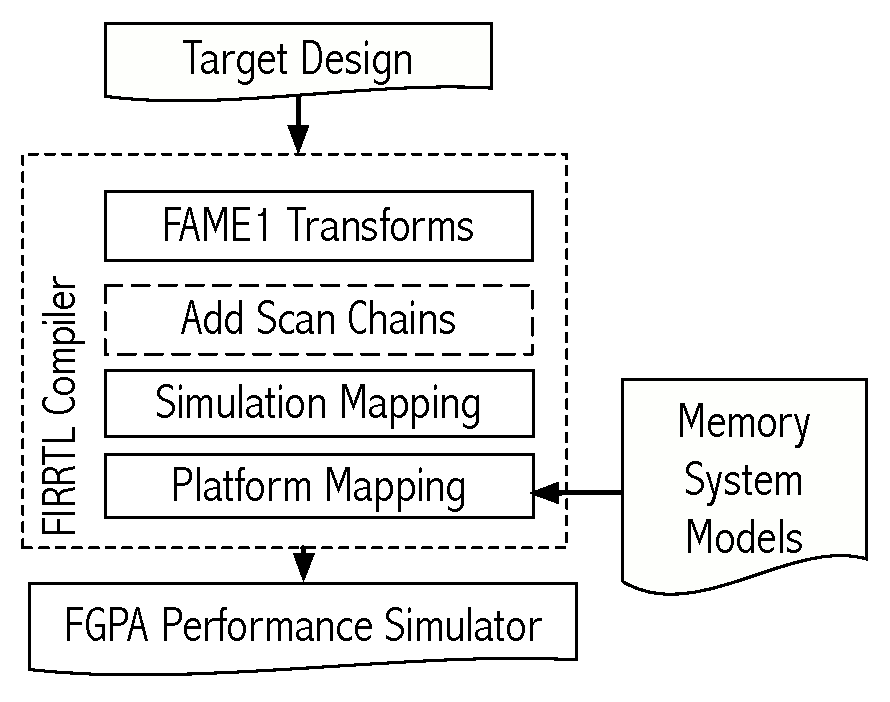
\includegraphics[width=7cm]{figures/firrtl.pdf}
	\caption{FIRRTL custom transforms for the FPGA simulator}
	\label{fig:firrtl}
\end{figure}

\section{Host-Target Decoupling in MIDAS}






\section{Transformations of Source RTL}

MIDAS uses FIRRTL compiler passes to preform transformation source RTL into
host-decoupled models. The most important of these is the FAME-1
transformation, which adds to requsite logic to host-decouple target RTL, so
that it may conform to a RAMP model of execution. \TODO{See Section}. In figure
\TODO{Auto-transformation} below, the procedure through which source RTL is
host decoupled is illustated.

Additional transformations may be invoked to add scan chains and I/O trace
buffers for debugging, and for state snapshotting for use with
Strober\cite{strober}.

\section{Platform Mapping}

\section{Target Machines}

While this approach is applicable to arbitrary RTL, one challenge lies in
sourcing the RTL to build a realistic target. While we build on RocketChip and
\RISCV, our approach could in principle be used with other open-source designs
such as OpenPiton\cite{openpiton} and FabScalar\cite{fabscalar}.

\section{Target Machines}
